\graphicspath{ {HW-PIC/} }


\chapter{Hardware}

    \section{Umsetzung - V1}
    
    In diesem Kapitel werden die unterschiedlichen Hardwarerevisionen des Projektes
    beschrieben. 

        \subsection{Versorgung}
        Das Board wird mit 5V über USB-C versorgt, um den ESP32-S3 mit 3V3 zu 
        versorgung, wird ein AMS1117 Spannungswandler verwenden. Dieser wurde ausgewählt, 
        aufgrund der einfachen Implementierung. Die Verluste bei der Umwandlung können vernachlässigt werden, da 
        es sich nicht um ein batteriebetriebenes Gerät handelt.

            \begin{figure}[h!]
                \centering
                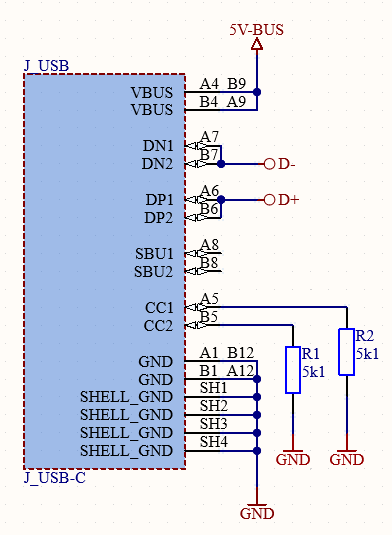
\includegraphics[width=7cm]{usb-c}
                \caption{USB-C Büchse "programmiert" mit Widerständen.}
                \label{fig:sch1}

            \end{figure}

        Die Widerstände R1 und R2 mit 5,1kOhm sind mit den CC-Leitungen auf GND verbunden.
        Dadurch weiß das Netzteil welche Spannung und wie viel Strom es zur verfügung stellen
        muss. 

            \begin{figure}[h!]
                \centering
                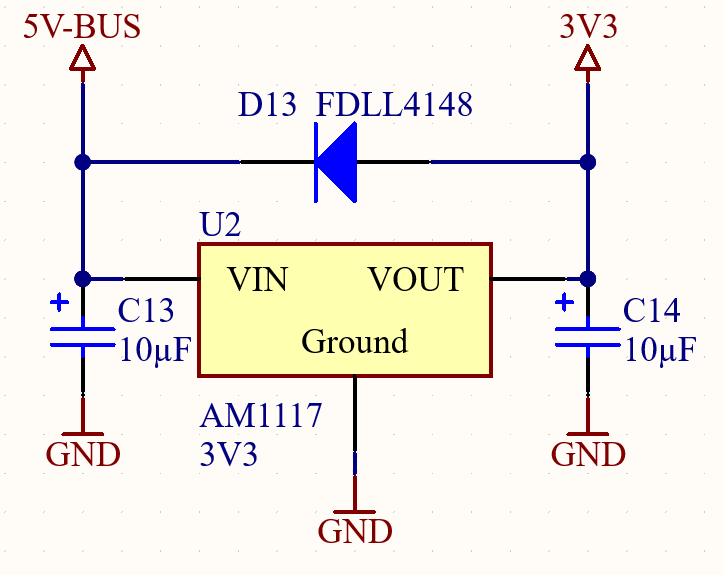
\includegraphics[width=8cm]{powersupply}
                \caption{AMS1117 mit 3V3 Ausgangsspannung.}
                \label{fig:sch2}
                
            \end{figure}

        Ein- und Ausgangsseitig liegt jeweils ein Glättungskondensator. Die Diode wurde hinzugefügt 
        um zu verhindern, dass am Ausgang eine größere Spannung
        anliegt als beim Eingang - wie z.B. beim Abstecken des Gerätes.

        \newpage

        \subsection{Mikrocontroller}
        Der ESP32-S3-WROOM-2 ist das Herzstück des Gerätes. Dieser verfügt über eine On-board PCB Antenne
        und kommuniziert darüber mit dem Smart-Home System. 

            \begin{figure}[h!]
                \centering
                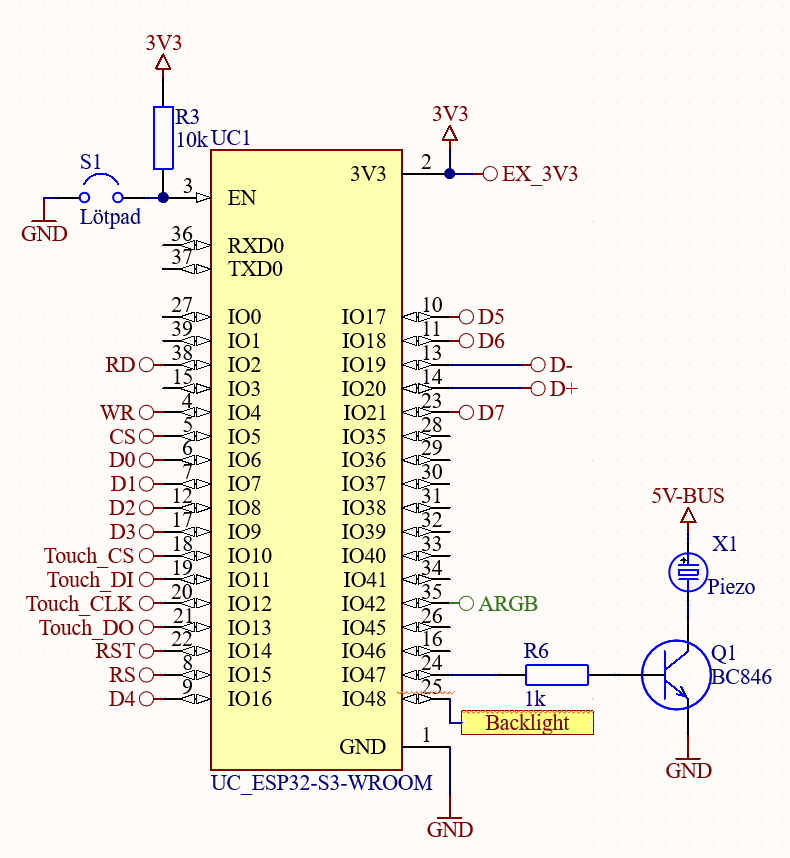
\includegraphics[width=8cm]{microcontroller.png}
                \caption{uC im Schaltplan.}
                \label{fig:sch3}

            \end{figure}

        \newpage
        \subsection{Display}
        Das Display wird parallel im 8-BIT Modus angesteuert. Die Pins mit denen 
        kommuniziert wird sind nicht fix in der Libary festgelegt und können am Esp32-S3 
        frei ausgewählt werden. 

            \begin{figure}[h!]
                \centering
                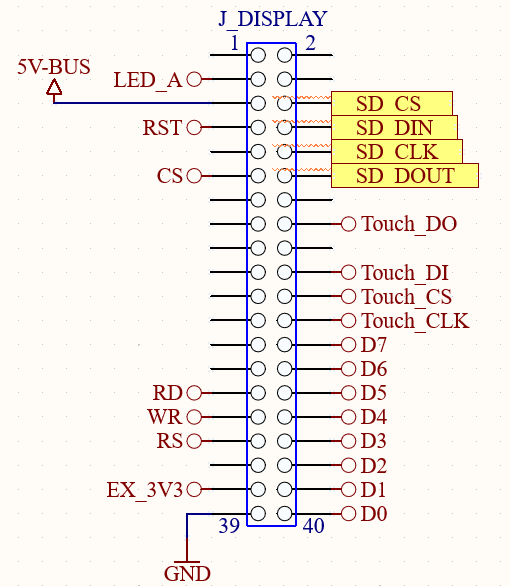
\includegraphics[width=8cm]{connector.png}
                \caption{Stecker für Display und Touch}
                \label{fig:sch4}

            \end{figure}

        Das Display wird über einen 40-Pin Stecker angeschlossen. Die Pins sind in der Abbildung \ref{fig:sch4}.
        Das zugekaufte Display hat eine Auflösung von 800x480 Pixeln und nutzt den SSD1963 Controller.
        Es ist ebenfalls ein SD-Kartenleser eingebaut. Dieser kann über SPI ausgelesen(Gelb markiert), ist 
        aber für dieses Projekt nicht in verwendung. 

        \newpage
        Das Display wurde über Amazon erworben.

            \begin{figure}[h!]
                \centering
                
\includegraphics[width=8cm]{TBD.png}
                \caption{Vorderseite des Displays.}
                \label{fig:displayfront}
            
            \end{figure}

            \begin{figure}[h!]
                \centering
                
\includegraphics[width=8cm]{TBD.png}
                \caption{Rückseite des Displays.}
                \label{fig:displayback}
            
            \end{figure}

        

        \newpage
        \subsection{Touch}
        Die Berührung am Resisivtouch-Panel wird vom XPT2046 erfasst und mittels 
        SPI-BUS vom µC ausgelesen. Da es bei der Implementierung von Touch softwareseitig
        Probleme gab, wurde stattdessen ein Drehgeber mit Taste verwendet.
        Dafür wurden die in der Abbildung \ref{fig:sch1} bzw. \ref{fig:sch4} gezeigten Pins mit 
        dem Prefix "Touch" für das Einlesen des Drehgebers verwendet.

        \subsection{LED-Streifen}

        Der LED-Streifen ist mit WS2812B bestückt. Das sind adressierbare RGB-LEDs, 
        die über einen einzigen Datenpin angesteuert werden. 
        Der Datenpin des LED-Streifens ist mit dem GPIO42 des ESP32-S3 verbunden. 

            \begin{figure}[h!]
                \centering
                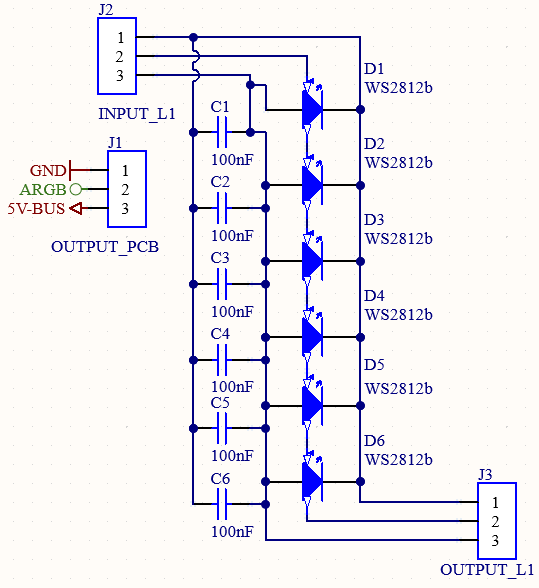
\includegraphics[width=10cm]{rgb.png}
                \caption{Anschluss und Beschaltung der LED-Streifen.}
                \label{fig:led_strip}
            \end{figure}

        % \subsection{PCB}



 
    \newpage
    \section{V1.1 (Finale)}       
    In diesem Kapitel der Hardware werden nur die Änderungen zur V1 beschrieben. 

        \subsection{Mikrocontroller}
        

            \begin{figure}[h!]
                \centering
                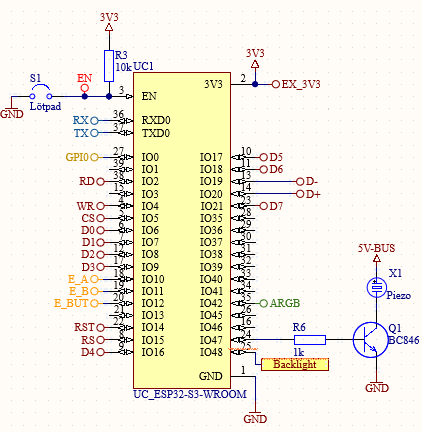
\includegraphics[width=12cm]{microcontroller-v1.1.png}
                \caption{Geänderte Schaltung.}
                \label{fig:sch5}

            \end{figure}

        Der Schaltplan wurde angepasst um den Rotary Encoder sowie das Serial-Interface auf
        einen Pin-Header legen zu können.

        \newpage
        \subsection{Rotary Encoder}
        Die Touch-Funktion wurde durch einen Drehgeber ersetzt. Dieser hat eine Taste und
        zwei Ausgänge für die Drehrichtung. Der Drehgeber wird an die Pins 'E\_A', 'E\_B' und 'E\_BUT'
        am ESP32-S3 angeschlossen. 

            \begin{figure}[h!]
                \centering
                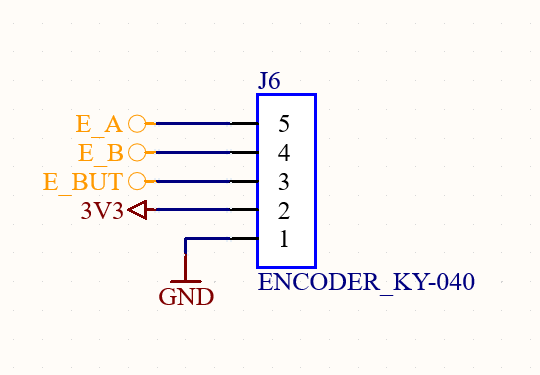
\includegraphics[width=6cm]{encoder.png}
                \caption{Anschluss: Drehgeber mit Taste.}
                \label{fig:sch6}

            \end{figure}

        
        
        Der Inkrementalgeber hat die relativen Ausgange A und B Signalen. Diese geben beide
        eine definierte Menge an Impulse ab. Beide Signale sind zueinander 90° Phasenverschoben. Somit
        kann die Drehrichtung bestimmt werden. Da je nach Drehrichtung die positive Flanke entweder
        zuerst bei A oder B erfasst wird.

            \begin{figure}[h!]
                \centering
                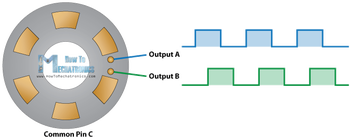
\includegraphics[width=10cm]{encoder_explain.png}
                \caption{Erklärung über Encoder von "How to Mechatronics"\cite{dejan_how_2016}}
                \label{fig:sch7}

            \end{figure}

            \begin{figure}[h!]
                \centering
                
\includegraphics[width=8cm]{TBD.png}
                \caption{KY-040 Encoder}
                \label{fig:sch8}

            \end{figure}
        Der Encoder KY-040 ist fertig bestückt auf ein PCB. Wie in Abbildung \ref{fig:sch6} zu sehen ist, 
        hat dieses Bauteil 5 Anschlussdrähte. Der Encoder gibt 20 Impulse pro Umdrehung aus.

        \newpage
        
        \subsection{Serial-Interface}
        Das Serial-Interface wurde auf einen Pin-Header gelegt um die Programmierung des ESP32-S3
        zu erleichtern. Bei der Entwicklung wurde festegstellt, dass beim programmieren 
        die Möglichkeit besteht, die Upload Funktion über USB unabsichtlich zu sperren. Neuer
        Code kann dann nur mehr über Serial hochgeladen werden. 

            \begin{figure}[h!]
                \centering
                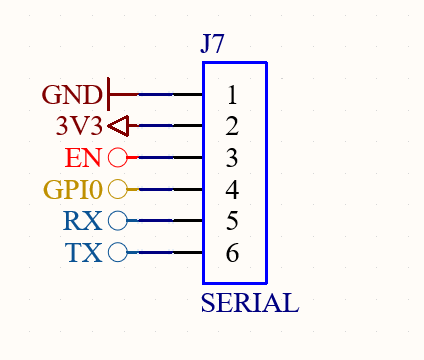
\includegraphics[width=8cm]{serial.png}
                \caption{Serial-Interface}
                \label{fig:sch9}

            \end{figure}
        
        Dieser Anschluss ist nur zum Programmieren und Debuggen gedacht.
    \newpage
    
    \section{PCB}

    In diesem Kapitel werden die unterschiedlichen PCBs beschrieben.


        \subsection{ARGB-Print}
        Dieser Print hat einen Eingang und einen Ausgang, es können mehrere von diesen 
        Platinen in Reihe geschalten werden.

        \begin{figure}[h!]
            \centering
            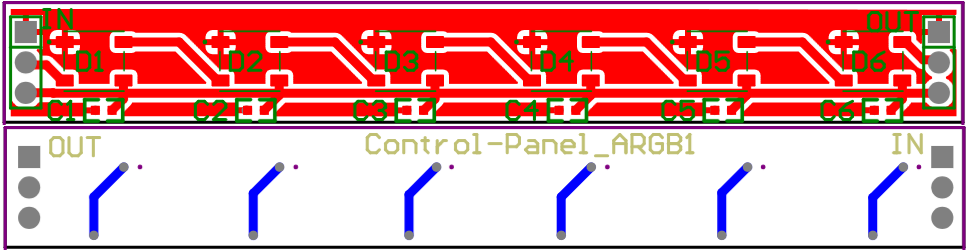
\includegraphics[width=8cm]{pcb-argb.png}
            \caption{PCB-ARGB wird blieb für V1.1 unverändert.}
            \label{fig:pcbargb}

        \end{figure}

        \subsection{V1}

        Das PCB ist so entworfen worden, damit es auf der Rückseite des Displays augesteckt 
        werden kann.

            \begin{figure}[h!]
                \centering
                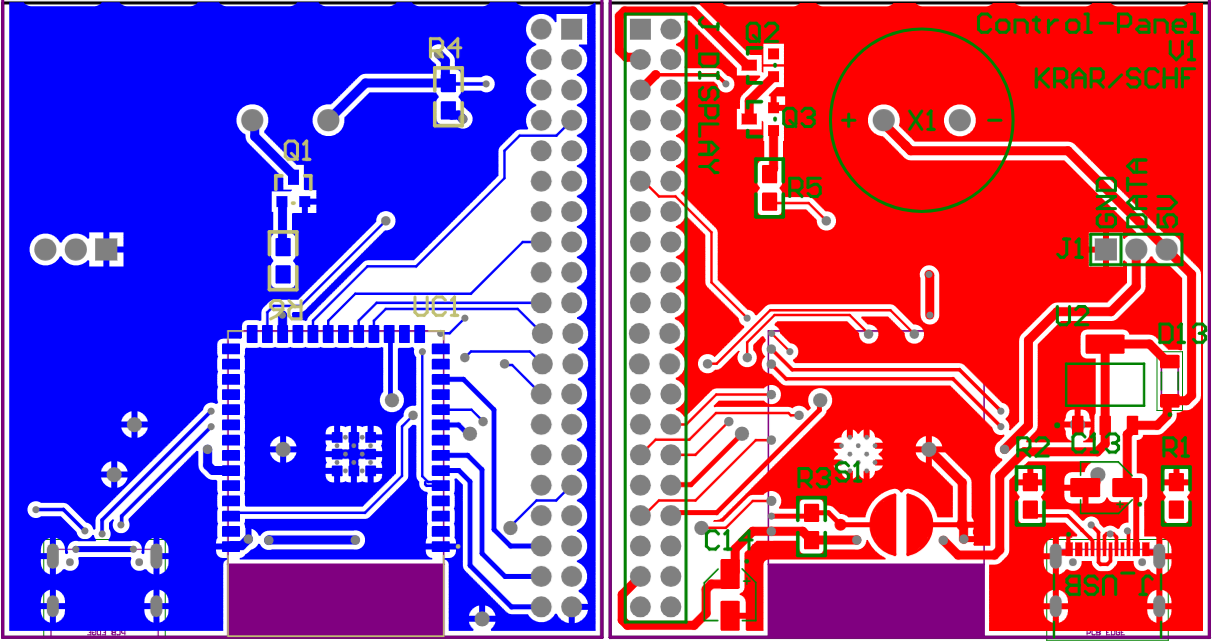
\includegraphics[width=12cm]{pcb-v1.png}
                \caption{PCB V1}
                \label{fig:pcb1}

            \end{figure}

        \newpage
        \subsection{V1.1}

        Das PCB wurde für die finale Version wurde angepasst. Der Rotary Encoder und das Serial-Interface
        haben jetzt einen eigenen Pin-Header.

            \begin{figure}[h!]
                \centering
                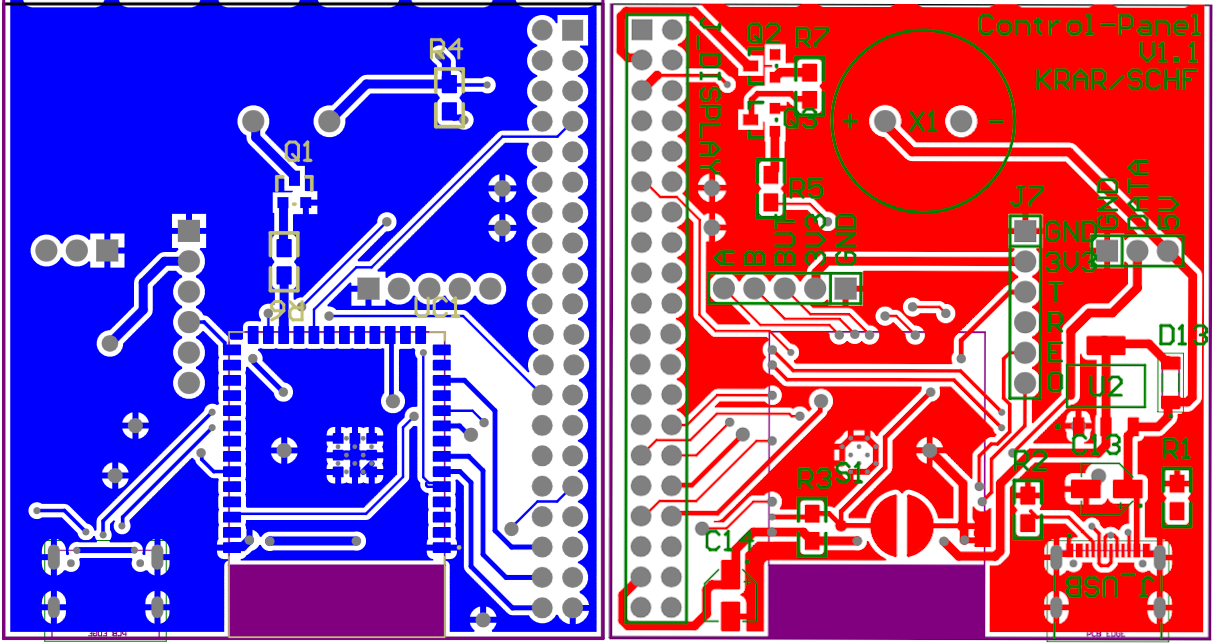
\includegraphics[width=12cm]{pcb-v1.1.png}
                \caption{PCB V1.1}
                \label{fig:pcb1.1}

            \end{figure}
            
        
    \newpage
    \section{Gehäuse}
    Das Gehäuse wurde aus 3D-gedruckten Teilen zusammengesetzt. Die Teile wurden in Fusion 360 
    entworfen und anschließend mit einem Creality Cr-10s Pro V2 gedruckt. Das Gehäuse besteht aus zwei 
    Hauptteilen: dem oberen und dem unteren Teil. Diese Teile werden durch Schrauben zusammengehalten.

        \begin{figure}[h!]
            \centering
            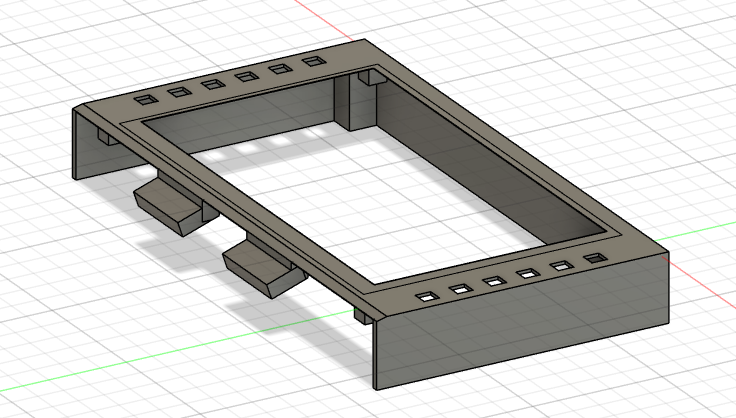
\includegraphics[width=10.5cm]{case_top.png}
            \caption{Oberes Teil des Gehäuses.}
            \label{fig:case_top}
        \end{figure}

    Der obere Teile des Gehäuses ist so gestaltet, dass es alle Komponenten sicher 
    haltet und gleichzeitig einen einfachen Zugang zu den Anschlüssen und Bedienelementen ermöglicht.
    Das Display und die LED streifen werden hier verbaut. 

        \begin{figure}[h!]
            \centering
            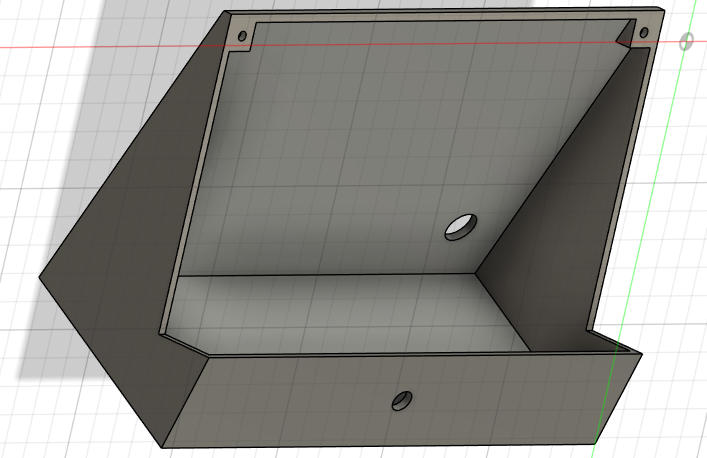
\includegraphics[width=9cm]{case_bottom.png}
            \caption{Unteres Teil des Gehäuses.}
            \label{fig:case_bottom}
        \end{figure}

    
    Der untere Teil des Gehäuses ist so gestaltet, dass der Oberteil sicher darauf sitzt und alle internen
    Komponenten schützt. Es bietet auch Öffnungen für die Stromversorgung. In dieses Teil wird
    die Strombuchse sowie der Encoder verbaut.
   

    % \newpage
    % \section{Fazit}
    % Die Hardware wurde in mehreren Iterationen entwickelt und getestet. Die finale Version erfüllt
    % alle Anforderungen und funktioniert zuverlässig im vorgesehenen Einsatzbereich. Durch die
    % Verwendung von Standardkomponenten und die sorgfältige Planung der Schaltungen konnte eine
    % robuste und kosteneffiziente Lösung realisiert werden. 

    